%%%%%%%%%%%%%%%%%%%%%%%%%%%%%%%%%%%%%%%%
%             PREÂMBULO
%
% Contém as configurações do arquivo e pacotes utilizados
%
%%%%%%%%%%%%%%%%%%%%%%%%%%%%%%%%%%%%%%%%

\documentclass[12pt, titlepage]{report} % Documento normal, formata o título

% Pacotes para formatação de matemática
\usepackage{amsmath, amssymb, amsthm} 

% Imagens
\usepackage{float} % Inclusão de imagens
\usepackage[export]{adjustbox} % Centralização de imagens e tabelas
\usepackage{subcaption} % Legendas
\graphicspath{fig/}

% Configurações da página
% A4, margens
\usepackage{geometry}
\geometry{
    a4paper,
    total={170mm,257mm},
    left=20mm,
    top=20mm,
}

% Configurações de espaçamento entre linhas e parágrafos
\usepackage{setspace}
\onehalfspacing{}
\usepackage{indentfirst}
\usepackage[skip=0pt, indent=1.25cm]{parskip}

% Alinhamento de texto (justificado)
\usepackage{ragged2e}
\justifying{}

% Configura a hifenização em português 
\usepackage[portuguese]{babel}
\addto\captionsportuguese{
    \renewcommand{\contentsname}{Sumário}
}

% Coloca o número de página no lugar certo
\usepackage{fancyhdr}
\pagestyle{fancy}
\fancyhf{}
\renewcommand{\headrulewidth}{0pt}
\fancyhead[R]{\thepage}

% 
\fancypagestyle{plain}{%
    \fancyhf{} % clear all header and footer fields
    \fancyhead{} % clear all header fields
    \fancyfoot{} % clear all footer fields
    \fancyhead[R]{\thepage}
    \renewcommand{\headrulewidth}{0pt}
    \renewcommand{\footrulewidth}{0pt}
}

% \usepackage[utf8]{inputenc} %% NECESSÁRIO c/ `pdflatex`
\usepackage{blindtext}
\usepackage{hyphsubst}

% Gerador de citações
% Configurado para o estilo ABNT na bibliografia final, 
% e citações indiretas indexadas numericamente
%
% Vai usar o arquivo refs.bib como fonte
\usepackage[nottoc,numbib]{tocbibind}

\usepackage[style=abnt, backend=biber, sorting=nty]{biblatex}
\addbibresource{./1.bib}
\setlength\bibitemsep{0.5\baselineskip} % espaçamento entre itens da bibliografia
\AtBeginBibliography{\singlespacing}

% Seleciona Times New Roman como a fonte desejada
\usepackage{fontspec}
\setmainfont{Times New Roman}

% Configura os comandos \url{} e \ref{}, sendo o último para citações dentro do arquivo (e. g. "Veja \ref{introdução}")
% \usepackage[hidelinks,colorlinks=true,linkcolor=blue,citecolor=blue,urlcolor=blue]{hyperref}
\urlstyle{same}

% Listas com enumerações
\usepackage{enumitem}
\setlist{nosep}
\usepackage{flafter}

\usepackage{tabularx, booktabs}

\usepackage{array}

\usepackage{changepage}

\usepackage{csquotes}

\usepackage{epigraph}
\setlength\epigraphrule{0pt}


\usepackage{calc}


% Dados técnicos.
\usepackage{titling}
\title{Por que privacidade?\\A proteção de dados pessoais num mundo conectado}
\author{Francisco Pessoa}
\date{São Paulo\\2025}

\usepackage{titlesec}
\titlespacing{\chapter}{0pt}{0pt}{1.5\baselineskip}
\titlespacing{\section}{0pt}{1.5\baselineskip}{1.5\baselineskip}
\titleformat{\chapter}[display] {\normalfont\Huge\bfseries\singlespacing}{\chaptertitlename\ \thechapter}{0pt}{\Huge}

\interfootnotelinepenalty=10000

\usepackage{quoting}

\quotingsetup{
    leftmargin=4cm,
    rightmargin=0cm,
    vskip=\baselineskip,
    font={small}
}

\AtBeginEnvironment{quoting}{\singlespacing}

\usepackage[hang,flushmargin]{footmisc}

\hyphenation{Facebook}
\hyphenation{Twitter}
\hyphenation{Meta}
\hyphenation{Google}
\hyphenation{Analytics}
\hyphenation{Internet}

\begin{document}
\setlength \epigraphwidth {\textwidth-7cm}
\begin{titlepage}
\begin{center}
\vspace*{3\baselineskip}
\textbf{Colégio Ítaca}

\vspace{4\baselineskip}

\textbf{\theauthor}

\vspace{10\baselineskip}

\thetitle

\vspace{5\baselineskip}
\end{center}

\begin{flushright}

{\small
Professor Orientador\\João Homero do Amaral}
\normalsize

\vspace{4\baselineskip}

\end{flushright}

\begin{centering}

\onehalfspacing
\normalsize
\thedate

\end{centering}
\end{titlepage}

\newgeometry{
    top=3cm,
    bottom=2cm,
    left=3cm,
    right=2cm
}

\tableofcontents
% \newpage
% \listoffigures

\chapter{Os olhos que tudo vêem: caracterizando a coleta de dados}

\epigraph{\justifying{

\itshape A coisa seguia fazendo o que tinha que fazer, independentemente do que ele quisesse.
Registrava minúsculas diferenças ao redor dele, uma ligeira alteração na umidade, uma fração de decréscimo na temperatura, o progresso de um inseto no teto da tendestiladora, a aproximação solene do amanhecer no trecho estrelado do céu que ele enxergava pelo lado transparente da tenda.
}}{---Frank Herbert, \textit{Duna}}

Conforme a Pesquisa Nacional por Amostra em Domicílios (PNAD Contínua, realizada pelo Instituto Brasileiro de Geografia e Estatística), em 2023, 92,5\% das casas brasileiras tinham acesso à Internet. O folheto no qual o dado foi divulgado considera que ``apesar do aumento consistente desde o início da série histórica, essa taxa de crescimento tem sido cada vez menor, o que conversa com a aproximação desse número à universalização da Internet nos domicílios brasileiros'' \cite[p.6]{pnadcontínua_acesso_2024}.
Assim, mais do que nunca, a população brasileira está integrada em serviços online -- serviços esses que têm como uma de suas funções coletar quantidades massivas de dados pessoais.

Segundo \textcite{vopson_information_2020}, a cada ano, são gerados aproximadamente 7,3 \textit{zettabytes} de dados, isto é, $7,3\times10^{21}$ \textit{bytes}\footnote{Um \textit{byte} é formado por oito \textit{bits} -- oito ``uns ou zeros'' -- e é considerado a menor unidade de informação para um computador.}. 
Essa quantidade estrondosa de informação não é constituída só de vídeos, textos, imagens, entre outros; a título de referência, o \textit{Internet Archive}, organização sem fins lucrativos que busca arquivar todo o conteúdo publicamente disponível, tem um acervo na ordem dos \textit{petabytes}, ou seja, $10^{15}$ \textit{bytes} \cite{internetarchive_petabox_}. 
Isto é, esse acervo, que busca salvaguardar todos os livros, \textit{sites}, filmes, seriados e documentos em livre acesso, inclusive compreendendo sites que estão hoje fora do ar, tem tamanho equivalente a $0,0001\%$ ou um milionésimo dos dados gerados \textit{por ano}.

Na verdade, o resto desse volume gigantesco é, em sua maioria, composto por registros cotidianos, resultados da interação rotineira dos usuários com serviços \textit{online}.
Eles são visualizações, \textit{likes}, trajetos de mobilidade, ingressos, compras, saldos, histórico de buscas, entre muitos outros \cite{cyphers_oneway_2019}.
Esses dados não são individualmente importantes; só adquirem significado no conjunto, na criação de um \textit{perfil de comportamento} individual.
\textcite{youyou_computerbased_2015} demonstraram que, tomando como base informações aparentemente inofensivas -- amizades do \textit{Facebook} -- é possível criar modelos computacionais que fazem previsões melhores, ou seja, sabem mais sobre o comportamento de uma pessoa do que parentes e amigos próximos.
De modo similar, infere-se posicionamento político, localização, hábitos de consumo, interesses midiáticos e outra multitude de características pessoais extremamente valiosas partindo desses dados.
O modo de funcionamento desses modelos é tratado no capítulo 2 deste texto.

Esses dados estão na mão, principalmente, das grandes empresas de tecnologia responsáveis pela maioria do tráfego na Internet.
Ainda segundo \textcite[p.~23]{cyphers_oneway_2019}, a Google rastreia por volta de 80\% de todas as transações na rede. 
Isto é, fica sabendo de 4 a cada 5 requisições. Atrás dela figuram outras grandes empresas como Facebook, Yandex (russa), Amazon, Microsoft e Adobe. 
Isto não implica necessariamente em tráfego direto: não são 80\% das solicitações que acontecem em domínios
\footnote{Um domínio é um nome de site na internet, em posse de uma pessoa ou organização. Por exemplo, o Instagram é dono do domínio instagram.com, e a USP, de usp.br. De um único domínio podem surgir subdomínios, como jornal.usp.br} da Google; contudo, em alguma etapa do processo, a Google estará envolvida.
Na maior parte do tempo, isso ocorre indiretamente, por meio de anúncios e \textit{iframes}\footnote{Um iframe é uma maneira de incluir o conteúdo visual de um site em outro, embutindo-o. É frequentemente utilizado para incluir postagens de redes sociais em notícias, por exemplo. Deste modo, ao invés de uma imagem estática abre-se a possibilidade de interação diretamente do site continente. Funcionam como uma caixa, dentro da qual o conteúdo de um site será mostrado.}, partes de um site que são provenientes de outro servidor.

\section{Características técnicas da vigilância}
Para entender como ocorre esse rastreamento, será utilizado um exemplo anedótico que condensa algumas das práticas comuns.
Utilizando as ferramentas de desenvolvedor do navegador, é possível obter um registro de todas as requisições feitas quando o usuário entra em um site, como um arquivo HAR \footnote{``Acervo HTTP'', do inglês ``HTTP Archive''. Essencialmente, é uma grande lista de requisições HTTP feitas por um site, onde HTTP é o protocolo de transferência por trás da Internet.}.
Um arquivo desse tipo gerado em www.uol.com
\footnote{Esses dados foram capturados no dia 16 de maio de 2025, às 15h. O agente de usuário (conjunto de informações sobre si mesmo que o navegador manda para o servidor do qual quer requerir informações) do computador era ``\textit{Mozilla/5.0 (X11; Linux x86\_64) AppleWebKit/537.36 (KHTML, like Gecko) Chrome/136.0.0.0 Safari/537.36}''. Esse experimento pode ser facilmente reproduzido em qualquer navegador, desde que o mesmo não inclua nenhuma medida de bloqueio de anúncios ou rastreadores. Basta entrar na aba de ``Inspecionar'', na aba de Rede/Tráfego, e fazer uma captura.}, 
revela que simplesmente carregar a página inicial da UOL (um famoso portal de notícias brasileiro) implica em pelo menos 500 requisições.
O grande problema, contudo, está no fato de que a maioria delas não é diretamente feita para www.uol.com e seus subdomínios, mas sim, puxam códigos e informações de outros lugares -- outros domínios. 
Entre eles, nesse exemplo, figuravam muitos domínios da Google, incluindo o Google Analytics, ferramenta que serve para registrar as ações feitas pelo usuário na página, como entrar em uma notícia, clicar num anúncio, fazer uma pesquisa, entre outros.
Em decorrência disso, atos simples, como mover o cursor, já elevam esse total: esse sistema registra todas as interações que puder. 
Após 10 minutos com a página parada, a conta já tinha passado das 1100 requisições.
Isso não é uma peculiaridade da UOL, mas sim, um conjunto de práticas muito comuns que acontecem em quase todos os sites monetizados, ou seja, que tiram algum dinheiro das visitas.

Pode parecer estranho que, ao entrar no UOL, o computador envie dados para um terceiro.
O mecanismo por trás disso é que a UOL propositalmente embute pedaços de código alheios, os chamados Kits de Desenvolvimento de Software (SDKs, do inglês \textit{software development kit}), que tomam controle parcial do tráfego da página.
Os SDKs são utilizados para incluir serviços de terceiros, e podem tanto ser absolutamente necessários, como para garantir autenticação de usuários ou uma funcionalidade de pagamento, quanto para outros fins, como rastrear o comportamento de quem visita a página.
Eles geralmente tomam o formato de um grande arquivo de código compactado, feito não para ser legível, mas sim rápido de carregar e executar.
Esse obscurantismo tem outro efeito além de diminuir o tamanho do arquivo: ele acaba por, ainda que não intencionalmente, dificultar a análise do seu conteúdo.

SDKs são muito usados para carregar anúncios.
Assim, ao invés de cada site tomar para si o trabalho de encontrar anunciantes, essa função é delegada para um serviço especializado, como o Google Ads.
Em troca, obtém-se dinheiro pelos anúncios e dados das interações com a página, a fim de saber quantos usuários clicaram em cada reportagem, se passaram um bom tempo lendo, entre outros -- tudo a fim de otimizar a monetização.

Uma ferramenta de monitoramento comumente utilizada são os chamados \textit{tracking pixels}, pequenos pontos da tela, invisíveis e indiferenciáveis, que acompanham movimentações do cursor.
Eles são registrados como um elemento da página, ganhando assim o privilégio de obter uma série de informações, mesmo sem que o usuário interaja com eles.
Seu uso é comum também em e-mails \cite{kelion_spy_2021}.
Outros sistemas de captura de dados não precisam reservar um pedaço da tela, ou seja, adquirir uma aparência física: é perfeitamente possível que esse rastreamento seja feito completamente por ``debaixo dos panos'', na forma de códigos que rodam paralelamente, em plano de fundo, sem interferir em nada na experiência principal da página.

Nesses casos, ainda é possível perceber que esse tipo de vigilância ocorre por meio da interceptação de requisições, como foi feito aqui com a UOL.
Com essa técnica, um grupo de pesquisa internacional formado por acadêmicos do instituto espanhol IMDEA, da Universidade Católica da Lovaina (KU Leuven, na Bélgica) e da Universidade Radboud de Nimega (na Holanda) descobriu que a Meta, empresa por trás do Instagram e do Facebook, abusava de uma vulnerabilidade de segurança no sistema operacional Android para coletar o histórico de navegação dos usuários, até passando por cima de recursos de segurança como a ``guia anônima''.
Essa funcionalidade estava escondida no Meta Pixel, um SDK de monitoramento, sem que os sites que usufruíam desse sistema soubessem. 
O Meta Pixel foi desativado depois dessa descoberta \cite{girish_disclosure_2025, teixeira_meta_2025}.

Outra prática que acontece no UOL, mas que também é amplamente difundida em outras páginas, é a do \textit{leilão de anúncios em tempo real}. 
Isso é uma prática organizada que determina \textit{qual} anúncio mostrar para um usuário que acessa aquele serviço, por meio de um leilão que dura poucos milissegundos.
Os anunciantes dão seus lances baseados em pacotes de dados do usuário-alvo que o \textit{site} (chamado de \textit{supply side platform} ou SSP, a plataforma de oferta) distribui.
O maior lance (dado pela \textit{demand side platform} ou DSP, a plataforma de demanda) ganha o espaço para disponibilizar seu anúncio.
Nesse meio tempo, esses dados já foram distribuídos para muitos potenciais clientes, que não necessariamente fizeram um lance.
Pode ocorrer que um dos participantes do leilão nem sequer tenha interesse em vender um anúncio, sempre dando lances inviáveis e se aproveitando disso para coletá-los.
Há amplos problemas éticos com esse sistema, que ocorre geralmente sem que os usuários saibam que seus dados estão sendo vendidos \cite{bashir_privacy_2019}: é a troca indiscriminada de informações pessoais por dinheiro como método de maximizar o lucro.

A monetização de dados não passa necessariamente pela venda de anúncios.
Está se tornando cada vez mais comum o uso de perfis de direção por seguros de carros \cite{mckinsey_monetizing_2016, hill_automakers_2024}.
Deste modo, o valor do seguro pode aumentar quando for entendido que o motorista dirige ``perigosamente'', segundo uma definição de perigo arbitrária e não revelada para o cliente.
Por meio da coleta de dados, o seguro consegue ter uma imagem compreensiva do motorista, e recalibrar-se nos moldes dessa imagem.
Assim, o motorista se vê coibido a exibir um tipo de comportamento, e forçado a dar para um terceiro um dado muito sensível: a localização em tempo real.

\section{Os indivíduos sob os olhos da vigilância}

Essa capacidade de caracterização -- traçar um perfil comportamental de alguém baseado em suas interações cotidianas -- é onde reside o perigo dessa vigilância.
Ela trata o ser humano como um modelo fechado, previsível.
Ademais, esses modelos, principalmente aqueles treinados com maiores quantidades de informação, são excelentes nessa tarefa, de modo que resultam em perfis acurados e ricos em detalhes.
Isso pode ser usado para, por exemplo, desencorajar mulheres que buscam aborto com propaganda direcionada \cite{coutts_antichoice_2016}, algo que só é possível pois algoritmos de classificação conseguiram identificar essas pessoas em específico dentre o universo de indivíduos.

É frequentemente dito que a Internet é um espaço anônimo, de modo que o que é feito nela é dificilmente ligado de volta a um indivíduo físico. 
Contudo, existe um grande problema com essa abordagem: mesmo sem as informações que podem identificar alguém 
-- endereço, número de identidade, conta bancária, que geralmente são mais contempladas em leis de proteção e privacidade, tornando sua aquisição e uso mais complicado -- 
elas podem ser facilmente deduzidas, quando necessário.
Os padrões de deslocamento, obtidos por aplicativos de GPS como o Google Maps, Waze e Moovit podem informar, com alguma precisão, o bairro, a rua, e até mesmo a casa onde alguém mora.
Pesquisas por produtos em sites de comércio eletrônico dão base para a dedução de hábitos de consumo e renda.

Essas informações precisam ser unificadas, isto é, que várias fontes de dados conversem entre si, para construir um perfil único e mais completo.
Isso requer diferenciar os usuários, algo que pode ser feito por qualquer tipo de identificação imutável do dispositivo em que esse acesso está sendo feito.
Por exemplo, são usados aqui o número de IP \footnote{O endereço de Protocolo de Internet (do inglês \textit{Internet Protocol adress}) é um identificador de dispositivo dado a ele pela operadora de Internet. Geralmente, é dado só um IP para o roteador, que serve para todos que estejam nele. É uma informação de fácil obtenção, pois qualquer conexão entre dois computadores envolve a troca de seus respectivos IPs. Os endereços de IP são controlados pelo provedor de Internet, e mudam ocasionalmente.}, endereço MAC \footnote{O número de Controle de Acesso ao Meio (do inglês \textit{Medium Acess Control adress}) de modo similar ao IP, é também utilizado para estabelecer a conexão entre dois computadores. Contudo, o endereço MAC vem embutido no dispositivo, e só é utilizado para conexões a cabo, sendo de mais difícil obtenção.}, os identificadores para anúncios providenciados pelo sistema operacional \footnote{Tal qual o {``Android Ad ID''} e o {``Apple IDFA''}.} e, ocasionalmente, um conjunto de informações enviadas pelo navegador no cabeçalho da requisição, algo conhecido como \textit{impressão digital de navegador}, do inglês \textit{browser fingerprinting} \cite{ohm_broken_2009, chen_fingerprinting_2019}.
Outras técnicas de identificação incluem registrar chaves criptográficas \cite{sy_tracking_2018} e obter nomes de redes de WiFi \cite{binder_republican_2019}.
Voltando ao exemplo anterior do Meta Pixel, as informações do histórico obtidas por meio da vulnerabilidade eram cruzadas com outras por meio do endereço de IP, de modo que Meta não só tinha essa informação, como também alguém a quem ela pertencia.
Detalhes dessas e mais técnicas podem ser encontrados em \textcite{cyphers_oneway_2019}.

Fundamentalmente, essa situação é um problema de confiança.
Podemos confiar em empresas que sabem de nossa personalidade e hábitos a fundo?
Se ainda não ficou claro pelos exemplos anteriores, não: dentro da coleta de dados opera suprema a lógica do capital, do lucro; sempre buscando novos mercados onde se expandir.
É por isso que são tão debatidas regulamentações legais do rastreio digital, algo que será melhor explorado no capítulo 3.
Por ora, basta entender que a coleta de dados tem como objetivo primeiro o lucro e depois o interesse dos seus usuários: é necessário se preocupar com serviços vendendo localização em tempo real \cite{mackey_eff_2019}, com informações de crianças sendo usadas para treinar Inteligências Artificiais \footnote{As Inteligências Artificiais serão expandidas no segundo capítulo. Por enquanto, é suficiente entender que são um tipo de algoritmo que precisa ser treinado, processo que necessita de uma grande quantidade de dados.} (doravante, IAs) \cite{schurig_meta_2024}, e com empresas rastreando as lojas que um consumidor frequenta \cite{soltani_privacy_2015}, além dos já citados problemas com seguros de carro, pois essas atividades são \textit{extremamente lucrativas}.

Em 2021, a ViaQuatro, operadora privada da Linha 4 - Amarela do metrô de São Paulo, foi multada por coleta ilegal de dados.
O Instituto de Defesa do Consumidor (Idec), que protocolou o processo, alegava uso indevido da tecnologia de reconhecimento facial por meio de câmeras embutidas nas portas de plataforma que filmavam a reação dos passageiros quando expostos a anúncios.
Concomitantemente, o sistema também estimaria gênero e idade.
\cite{soprana_viaquatro_2021}.
Isso é, de maneira muito clara, uma tentativa de otimizar o serviço de propaganda.
A \textit{otimização} é um fator muito importante aqui -- é, novamente, um tratamento matemático das relações humanas, de modo que a compra torna-se uma função que se deve maximizar.

\section{Vigilância política}

Os exemplos colocados aqui são principalmente relacionados às empresas estadunidenses, ou pelo menos ao que podemos hoje considerar um bloco tecnológico-econômico ocidental.
Não é possível falar disso sem mencionar a questão territorial: muitos desses serviços e produtos são provenientes do chamado ``Vale do Silício'', e compartilham filosofias semelhantes.
São essenciais os processos históricos que aconteceram concomitantes ao surgimento da Internet, principalmente, a instauração do neoliberalismo como sistema econômico hegemônico.
Para o economista bielorrusso Evgeny Morozov, em seu ensaio ``Capitalismo Tecnológico e Cidadania'', a retórica do Vale do Silício se espalhou globalmente graças ao ``triunfo da ideologia neoliberal subsequente à Guerra Fria que suprimiu com êxito os aspectos não econômicos da nossa existência social, fazendo com que a identidade de consumidor sobrepujasse a de cidadão'' \cite[p.~19]{morozov_big_2018}.
Não dá para dizer que a coleta de dados não seja praticada na Rússia ou na China -- ela é ubíqua mesmo dentro desses países -- mas é possível dizer que os mecanismos sociais de vigilância são inseparáveis da realidade econômica dos países onde acontecem.

Ainda segundo \textcite[p.~15]{morozov_big_2018},

\begin{quoting}
    Não há como responder a tais questões sem antes admitir a presença do elefante na sala do servidor: as nossas tecnologias - e as ideologias que elas promovem - são, em grande medida, norte-americanas. 
    É bem verdade que as empresas russas e chinesas têm fortalecido cada vez mais a sua musculatura, tanto em casa como no exterior. 
    Não há como negar, porém, que os governos desses países se opõem mais ao imperialismo de Washington do que ao neoliberalismo do Vale do Silício. 
    O que eles mais temem é o uso geopolítico das plataformas estrangeiras de tecnologia contra seus interesses nacionais; mas não veem muito problema no modelo básico hipercapitalista de plataforma/monopólio adotado por muitas empresas do Vale do Silício. 
\end{quoting}

Essa tal ``retórica do Vale do Silício'' trata-se principalmente de uma promessa de emancipação: tal como a Uber, que promete a seus usuários liberdade na mobilidade, ou mesmo as redes sociais, que prometem liberdade de expressão.
Ela é cuidadosamente feita para se passar por \textit{anti-establishment}; a Uber contra os taxistas, as redes sociais contra a grande mídia, a Airbnb contra os hotéis.
Contudo, é precisamente por meio dessa aparência `do contra' que o Vale do Silício consolidou novos monopólios, passou por cima de regulações trabalhistas existentes (e, assim, precarizou o trabalho), e, explorando o que por muito tempo foi uma terra-sem-lei de regulamentações -- o mundo digital -- impôs a vigilância como modelo básico de funcionamento.
É importante entender, pois, que ela constitui um discurso ideologicamente carregado, que normatiza uma ordem social específica -- a vigilância.

Essa vigilância opera como uma alienação de alguns aspectos da vida humana, que são terceirizados para esses algoritmos, de modo que ocorre uma aproximação entre modo de vida e o lucro.
Assim, cada ínfimo detalhe pode ajudar a monetizar mais um serviço, que -- por meios imorais e frequentemente danosos -- otimiza-se para extrair o máximo de dinheiro possível. Segundo \textcite{mejias_data_2024}, ocorre uma aproximação entre a \textit{cognição} (processo de adquirir o saber, aqui caracterizado como a coleta e uso de dados) e a \textit{economia} (processo de lucro), que provocou o surgimento de uma infraestrutura visando o processamento de dados por meio do que chamam de setor econômico de quantificação social.

É importante ressaltar isso -- foi construída uma \textit{infraestrutura de vigilância}.
É mais do que algo local, que acontece só com um site ou outro: trata-se de uma profunda transformação socioeconômica que apropria-se da vida humana para a geração de dados.
As redes sociais, as tais ``plataformas digitais'', são baseadas em atividades que já existiam; falar (Twitter e Facebook), fotografar (Instagram), encontrar emprego (Linkedin), comer (Ifood), e até paquerar (Tinder).
Diferenciam-se dos antigos métodos de realizar essas mesmas atividades, pois agora coletam dados e otimizam seus serviços para o lucro por meio deles.

Essa abordagem, para o que se propõe, é ótima; os modelos treinados por meio de quantidades massivas de dados são muito bons no que fazem, como já foi dito.
Tão boa que nem mesmo a política institucional escapou dela, e cada vez mais as eleições são pautadas pela capacidade de utilizar-se dessas plataformas.
E para essas plataformas, não importa a veracidade nem a moral de uma notícia: por exemplo, as \textit{fake news} nada mais são do que notícias otimizadas, que dão mais dinheiro.
Concilia-se essa enorme contradição interna pois, independentemente do que é publicado, o dinheiro dos anúncios continua fluindo \cite{morozov_big_2018}.

Voltando à ilusão da Internet como um espaço anônimo, é comum dizer que aqueles que não têm nada a esconder não deveriam se preocupar com privacidade.
O problema com essa abordagem é que privacidade não se trata de segredos a serem escondidos, assim como um cofre guarda seus conteúdos.
O problema da privacidade, tal como ele é posto agora, é muito mais ardiloso do que isso.
Quando tantas relações sociais estão ``plataformizadas'' -- isto é, passíveis à acumulação de dados --, e em plataformas que respondem também a uma lógica capitalista de lucro, tendendo ao monopólio, o mundo digital deixa de ser democrático, livre, e se torna sujeito à influência, por meio dos algoritmos.
Hoje, muitos formam opiniões, adquirem produtos e mudam suas rotinas motivados (ainda que parcialmente) pelo que viram, ouviram e leram no plano digital.

Seria ingênuo pensar que essas plataformas são neutras, e atuam puramente como intermediárias.
Elas têm interesses políticos concretos, e, com tantos dados e saber sobre a vida das pessoas, ampla influência também.
Em 30 de maio de 2025, o Partido Liberal (PL), entre cujos filiados figura o ex-presidente Jair Bolsonaro, organizou um grande seminário sobre tecnologia, com participação de altos executivos de grandes empresas de tecnologia como Google e Meta. 
Segundo Sérgio de Souza, repórter do Intercept que cobriu o evento,

\begin{quoting}
    A mensagem era clara: as big techs estavam ali em peso, abençoando o evento e compartilhando com os participantes o “caminho das pedras” para usar suas ferramentas mais novas e poderosas.

    Essa relação de proximidade foi reforçada por Bolsonaro, que discursou no encerramento do encontro, aos gritos de “volta, capitão” vindos da plateia. O ex-presidente não deixou dúvidas ao afirmar que as empresas de tecnologia estavam ``do lado certo''. \cite{desouza_treinamento_2025}
\end{quoting}

Elas não estavam ali por acaso: vigiar é um ato profundamente político, que está entre as bases da sociedade moderna. 
O filósofo Byung-Chul Han propõe que o antigo regime disciplinar na base do capitalismo industrial, agora se transformou em um regime baseado em informação.

\begin{quoting}
    O capitalismo da informação, assentado sobre a comunicação e a conexão, torna obsoletas técnicas disciplinares como a isolação [\textit{sic}] espacial, a regulamentação rigorosa do trabalho ou o adestramento corporal. 
    A “docilidade” (\textit{Gelehrigkeit}, a capacidade de aprender, como em alemão se traduziu o termo francês \textit{docilité}), que significa também obediência ou ductilidade, não é o ideal do regime da informação. 
    O sujeito submisso do regime de informação não é nem dócil, nem obediente. 
    Ao contrário, supõe-se livre, autêntico e criativo. 
    Produz-se e se performa.
        
    [...]
    
    A dominação do regime de informação é ocultada, na medida em que se funde completamente com o cotidiano. É encoberta atrás da complacência das mídias sociais, da comodidade das máquinas de busca, das vozes embalantes das assistentes de voz ou da oficiosidade prestativa dos smart apps, os aplicativos inteligentes. O smartphone se revela como um informante eficiente, que nos submete a uma vigilância duradoura. [...] A
    vigilância infiltra-se no cotidiano na forma da conveniência. No presídio digital como zona de bem-estar smart não se ergue nenhuma oposição contra o regime dominante. O Like exclui toda revolução. \cite[p.~8-16]{han_infocracia_2022}
\end{quoting}

Han não é o único teórico que propõe que uma nova configuração do velho capitalismo está emergindo.
Alguns, inclusive, elencam um pós-capitalismo, chegando à ideia de tecnofeudalismo \cite{varoufakis_tecnofeudalismo_2023}.
Outros criticam essa elaboração, entendendo que há apenas uma continuação do sistema já existente \cite{morozov_nao_2023}.
Contudo, todos concordam que as tecnologias digitais estão provocando amplas transformações na nossa organização social e reorganizações produtivas.

Essas transformações já chegaram no Brasil: afora o congresso do PL já mencionado, nota-se o imenso embróglio político que acontece com as propostas de regulamentação de IAs e redes sociais no Legislativo, onde as grandes empresas de tecnologia exerceram muita pressão \cite{schurig_como_2024, schurig_quem_2024}.
Para o jornalista Sérgio Spagnuolo, ``O lobby das Big Techs venceu no Brasil'', de modo que as propostas que tinham potencial de as prejudicar, como o PL 2630/2020, foram engavetadas \cite{spagnuolo_lobby_2024}.

O Conselho Digital (https://conselhodigital.org.br/), entidade constituída por Amazon, Discord, Google, Hotmart, Kwai, Meta, TikTok e Uber é um dos expoentes disso.
As mesmas empresas que vigiam cada passo dado por seus usuários estão gastando muito dinheiro, fazendo um ``lobby descarado'' \cite{detoledo_pl_2023}, para garantir que projetos de lei onerosos a eles não sejam aprovados.
Chegaram ao ponto de até contratar o ex-presidente Michel Temer para atuar nas negociações \cite{mello_google_2023}.

Não é só no Brasil que isso acontece: na Nigéria, outro país não desenvolvido, ocorre um caso semelhante: a Meta não se contentou com as regulamentações propostas, e ameaça sair do país após receber uma multa milionária \cite{asadu_nigeria_2024}.

É importante reiterar que, hoje em dia, \textit{dados representam poder}: poder político, econômico, e social.
Ele permite uma maximização do lucro, efetivando uma subjugação dos processos sociais aos interesses financeiros de grandes corporações.

Um dos exemplos mais emblemáticos do uso de dados na política foi o caso da Cambridge Analytica, uma firma que realizava consultoria para campanhas publicitárias.
Por meio de dados de perfis do Facebook, que eles obteram por meio das ferramentas públicas do próprio Facebook, conseguiram criar perfis psicológicos de 50 milhões de usuários da plataforma e, assim, os servir anúncios especificamente criados para manipulá-los do jeito mais efetivo.
Com essa prática, chamada de anúncios escuros (do inglês \textit{dark ads}), uma publicidade será mostrada somente para aqueles que estão mais suscetíveis a ela, sendo praticamente invisível para o resto da sociedade.
A Cambridge Analytica foi parte integral da campanha eleitoral de Donald Trump em 2016, e dos partidários da saída do Reino Unido da União Europeia durante o Brexit.
Em ambos os casos, foi vitoriosa \cite{cadwalladr_50_2018}.

Por que é possível fazer isso?
Como até uma empresa de fora do Facebook consegue obter dados suficientes para fazer uma campanha tão destrutiva?
O caso da Cambridge Analytica ilustra alguns pontos bastante importantes.
Primeiro que é possível, por meio dos dados, criar modelos que descrevem com acurácia um eleitor, e, sem seu consentimento, manipulá-lo.
Quando marqueteiros falam de \textit{taxa de conversão} de um anúncio, poderiam muito bem estar falando da conversão de um voto.
Segundo Christopher Wylie, ex-funcionário da Cambridge Analytica, 
``Nós exploramos o Facebook para colher os perfis de milhões de pessoas. E construímos modelos para explorar o que já sabíamos sobre elas e atingir seus demônios interiores. Essa foi a base sobre a qual a empresa inteira foi construída.''
\cite[tradução~própria]{cadwalladr_50_2018}\footnote{No original, ``\textit{We exploited Facebook to harvest millions of people’s profiles. And built models to exploit what we knew about them and target their inner demons. That was the basis the entire company was built on.}''}

Segundo, que é possível e perfeitamente viável manipular eleições inteiras por meio dessas tecnologias, outorgando poder gigantesco àqueles que tiverem dinheiro para pagar por essas campanhas.
Tudo com conivência (ou, no mínimo, leniência) das grandes corporações de tecnologia.
E não precisa ser só em eleições: em 2018, uma investigação da ONU acusou o Facebook de ter tido um papel determinante no genocídio de mais de setecentos mil rohingyas muçulmanos no Myanmar \cite{barron_could_2018}.
O discurso de ódio, aos olhos do algoritmo de uma rede social, é só mais conteúdo viralizando, independente de quão intolerante for.
Ele dá dinheiro.

Capturar dados pessoais é um ato profundamente político.
E os usos que se dão a eles cada vez mais englobam o funcionamento da sociedade inteira.
Até agora, nesse texto, o algoritmo foi entendido como uma entidade elusiva e misteriosa, mas poderosa e influente.
Trata-se da \textit{maneira de processar} os dados coletados; o processo pelo qual as milhões de entradas em uma base de dados são transformadas em postagens recomendadas, anúncios, e tantas outras aplicações.
O próximo capítulo, assim, será dedicado a destrinchá-lo, compreender seus mecanismos de funcionamento, e entender como as técnicas de tratamento de dados que hoje são empregadas podem influenciar nos resultados, a partir de uma visão pautada na privacidade e na transparência.

\chapter{Título provisório do segundo capítulo}
É difícil ver o noticiário hoje sem se deparar com as Inteligências Artificiais (IAs).
Contudo, entre o uso de ChatGPT para trabalhos escolares, trabalhadores preocupados com perder o emprego para uma máquina, e até alguns com medo da humanidade ser inteiramente aniquilada num apocalipse da era digital, o uso de IAs é tão mais comum quanto mais dissimulado.

A culpa disso é do fato que ``Inteligência Artificial'' está muito mais próximo de uma expressão de marketing feita para atrair a atenção do que de um termo técnico.
Ela pressupõe uma semelhança entre o pensamento orgânico, tal como humanos o fazem, e um suposto pensamento sintético que, como há de ser visto nesse capítulo, é inteiramente dessemelhante a seu equivalente vivo.

Por trás da Inteligência Artificial há um conjunto de técnicas estatísticas e computacionais que fazem o chamado \textit{aprendizado de máquina} ou \textit{aprendizado estatístico}.
Antes de entender \textit{como} um computador pode aprender, é necessário responder \textit{por que} se quer que ele aprenda.
Há muito que um computador pode fazer sem a necessidade desse treinamento: isso inclui fazer contas, navegar pela Internet, assistir a um filme, tipografar uma monografia, entre outros.
Então, o que diferencia essas atividades de uma Inteligência Artificial?

A resposta é que essas atividades podem ser (e são) descritas por meio de código, o que requer representá-las como um conjunto de instruções claras e objetivas: uma receita de como as realizar.
É fácil elaborar uma receita de como reproduzir um vídeo, por exemplo.
O computador deverá localizar o arquivo que contém o vídeo, abri-lo, decodificá-lo e reproduzi-lo, convertendo as informações numéricas para cores a uma determinada taxa de vezes por segundo.
Por mais que cada passo aqui descrito possa ser desmembrado em tantos outros mais, qualquer programa de computador é descritível como um conjunto de instruções.
Todo processador é construído aos moldes de uma Arquitetura de Conjunto de Instruções (ISA, do inglês \textit{Instruction Set Architecture}), um modelo abstrato que delimita, simplificadamente, como se pode programá-lo.
Um dos componentes disso é um conjunto de instruções que o processador pode executar, para o qual \textit{todos} os programas que são usados devem ser reduzidos.
Essas instruções são coisas simples, como ``coloque tal valor em tal lugar'', ``some tal valor com tal valor'' e ``faça isso se tal valor for verdadeiro''.

É possível criar uma ``receita para escrever''?
Ou uma ``receita para recomendar vídeos''?
Isto é, um conjunto de instruções objetivas que permita realizar essas ações?
Não. 
E é aqui que entra o uso de uma IA: aproximar objetivamente processos que não podem ser descritos assim.

\section{Regressões Lineares}\label{sec:2:regres}
Observe o seguinte gráfico com o valor da anomalia da temperatura média do globo terrestre em relação à média do século 20, entre 1970 e 2025:

\begin{figure}[H]
    \centering
    \caption{Gráfico da anomalia (°C) em função do tempo (anos), 1970-2025}
    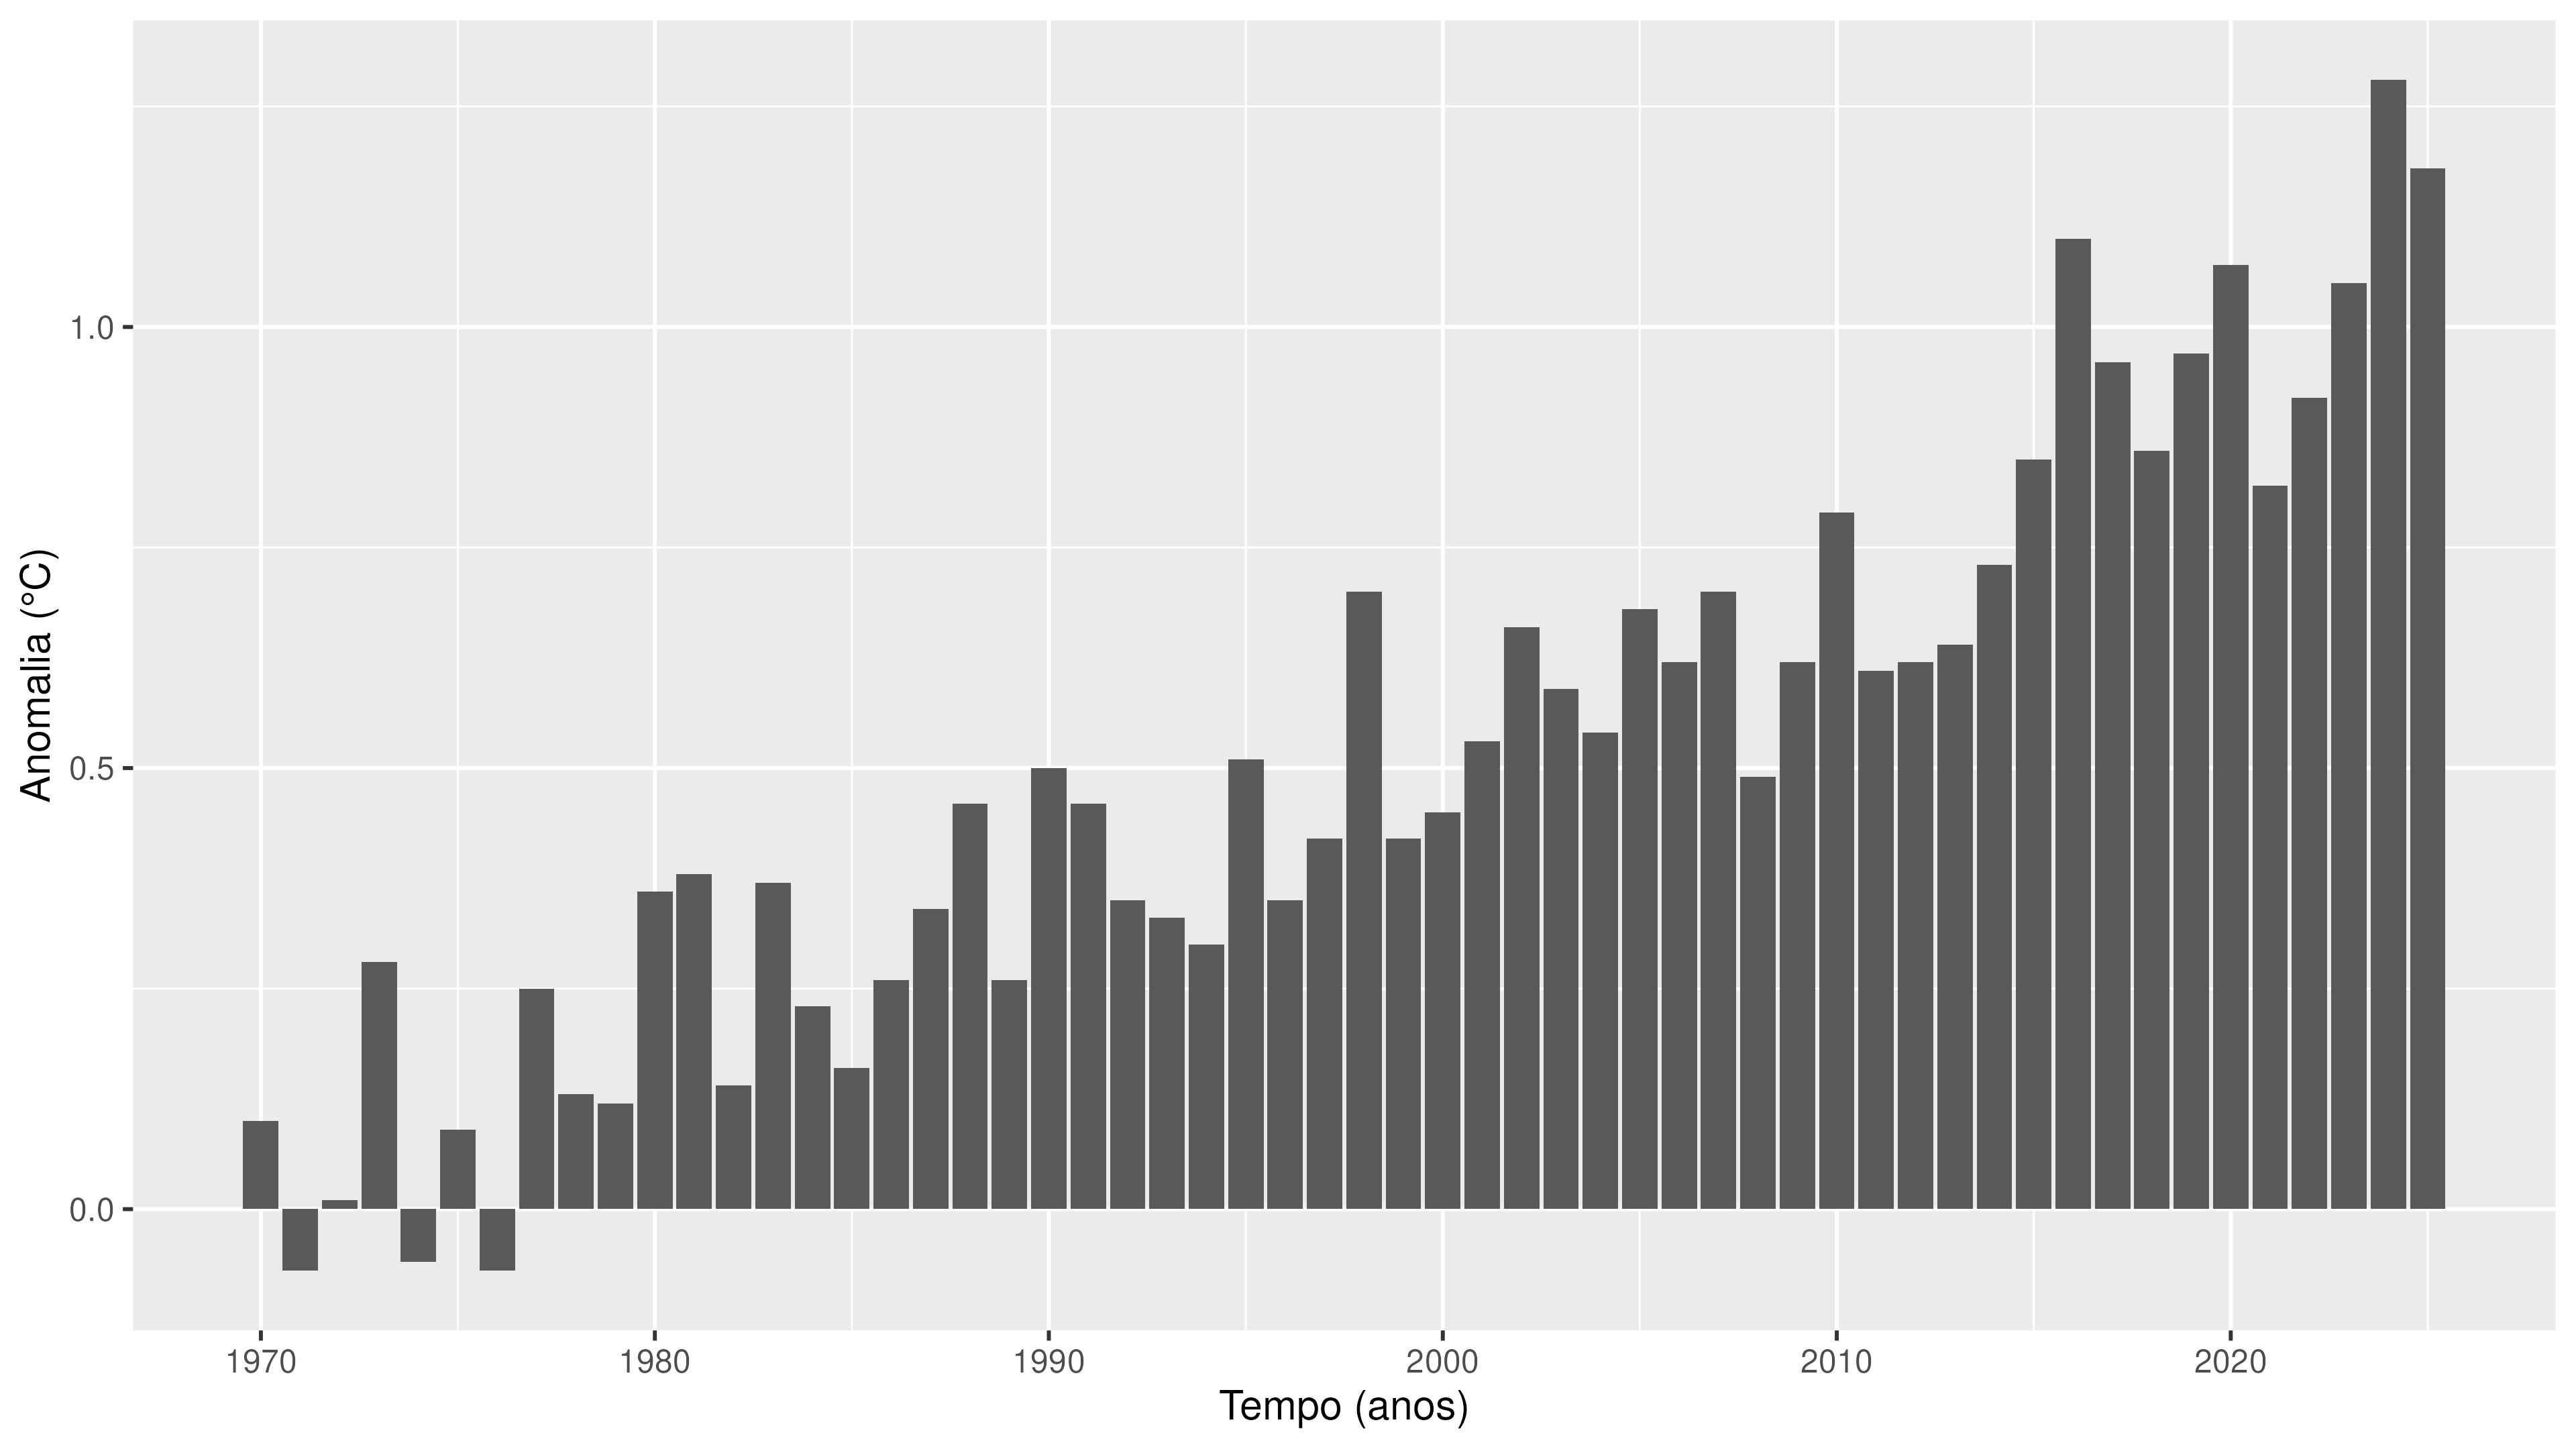
\includegraphics[width=\linewidth]{static/R/plot/anom-1-hist.png}
    \label{fig:2:anom-1-hist}
\end{figure}

Empiricamente, é possível perceber que existe uma tendência nesses dados, que seguem aproximadamente uma reta.
Porém, é difícil determinar precisamente de quanto é essa tendência, e para onde o gráfico continuará. 
Isso se deve ao fato de que o planeta Terra é um sistema complexo: ele não segue uma ordem do tipo ``aumente 0,5°C ao ano''.
Na metáfora da seção anterior, é impossível estabelecer uma receita para a temperatura do planeta em função do ano.

Pode-se, contudo, aproximá-la.
Sabe-se, a partir desses dados, como o modelo deve se comportar.
Não é possível, principalmente quando se trata de algo tão simples como uma reta, que ele abarque cada mínima mudança e inconsistência; é, afinal, uma aproximação.

Qual deverá ser a forma desse modelo?
Matematicamente, uma reta pode ser definida por meio de uma função linear, que, nesse caso, assumiria a forma de

\begin{equation}
A(t) = t\cdot\beta_1 + \beta_0
\end{equation}

Isto é, a anomalia $A$, em função do tempo $t$, pode ser definida como o tempo $t$ multiplicado por um coeficiente $\beta_1$ somado a um coeficiente estático $\beta_0$.
Assim, para determinar a anomalia, $t$ deve ser transformado, segundo os parâmetros $\beta_0$ e $\beta_1$ que, até agora, \textit{não se sabe quais são}.
Intuitivamente, $\beta_1$ é a inclinação da reta e $\beta_0$ a altura dela.
A grande pergunta, portanto, é quais são esses coeficientes, ou seja, como $t$ deve ser mudado para obter $A$.

Para determinar esses dois coeficientes, $\beta_0$ e $\beta_1$, é necessário primeiro conceber uma maneira de comparar dois modelos, e descobrir qual deles mais se aproxima do fenômeno aproximado.
Uma maneira muito simples de fazer isso é, para cada ano, contabilizar a distância entre o valor previsto pelo modelo e a observação real.
O objetivo da criação do modelo, assim, passa a ser reduzir ao máximo possível esse erro.
Comumente, ao invés de simplesmente usar o erro, é considerado o erro elevado ao quadrado; assim, erros menores são menos penalizados, e erros maiores serão ainda mais penalizados, pois seu valor crescerá com mais rapidez.
Essa abordagem é chamada de ``mínimos quadrados'', pois almeja minimizar os quadrados dos erros.

O processo de descobrir $\beta_0$ e $\beta_1$ é conhecido como \textit{aprendizado} ou \textit{treinamento}.
Ele envolve inicializar esses valores com um ``chute'', e, gradualmente, melhorá-los.
Para isso, muda-se ou $\beta_0$ ou $\beta_1$, incrementando-o por pouco. 
Se a mudança for bem-vinda, ou seja, diminuir o erro, ela é mantida; caso contrário, o original é melhor.
Ao repetir esse processo várias vezes, a reta será acomodada nos coeficientes com menor valor de erro.

No caso da figura \ref{fig:2:anom-1-hist}, isso toma a forma da figura \ref{fig:2:anom-3-scatter+reg}.

\begin{figure}
    \centering
    \caption{Gráfico da anomalia (°C) em função do tempo (anos), 1970-2025, com modelo de regressão linear}
    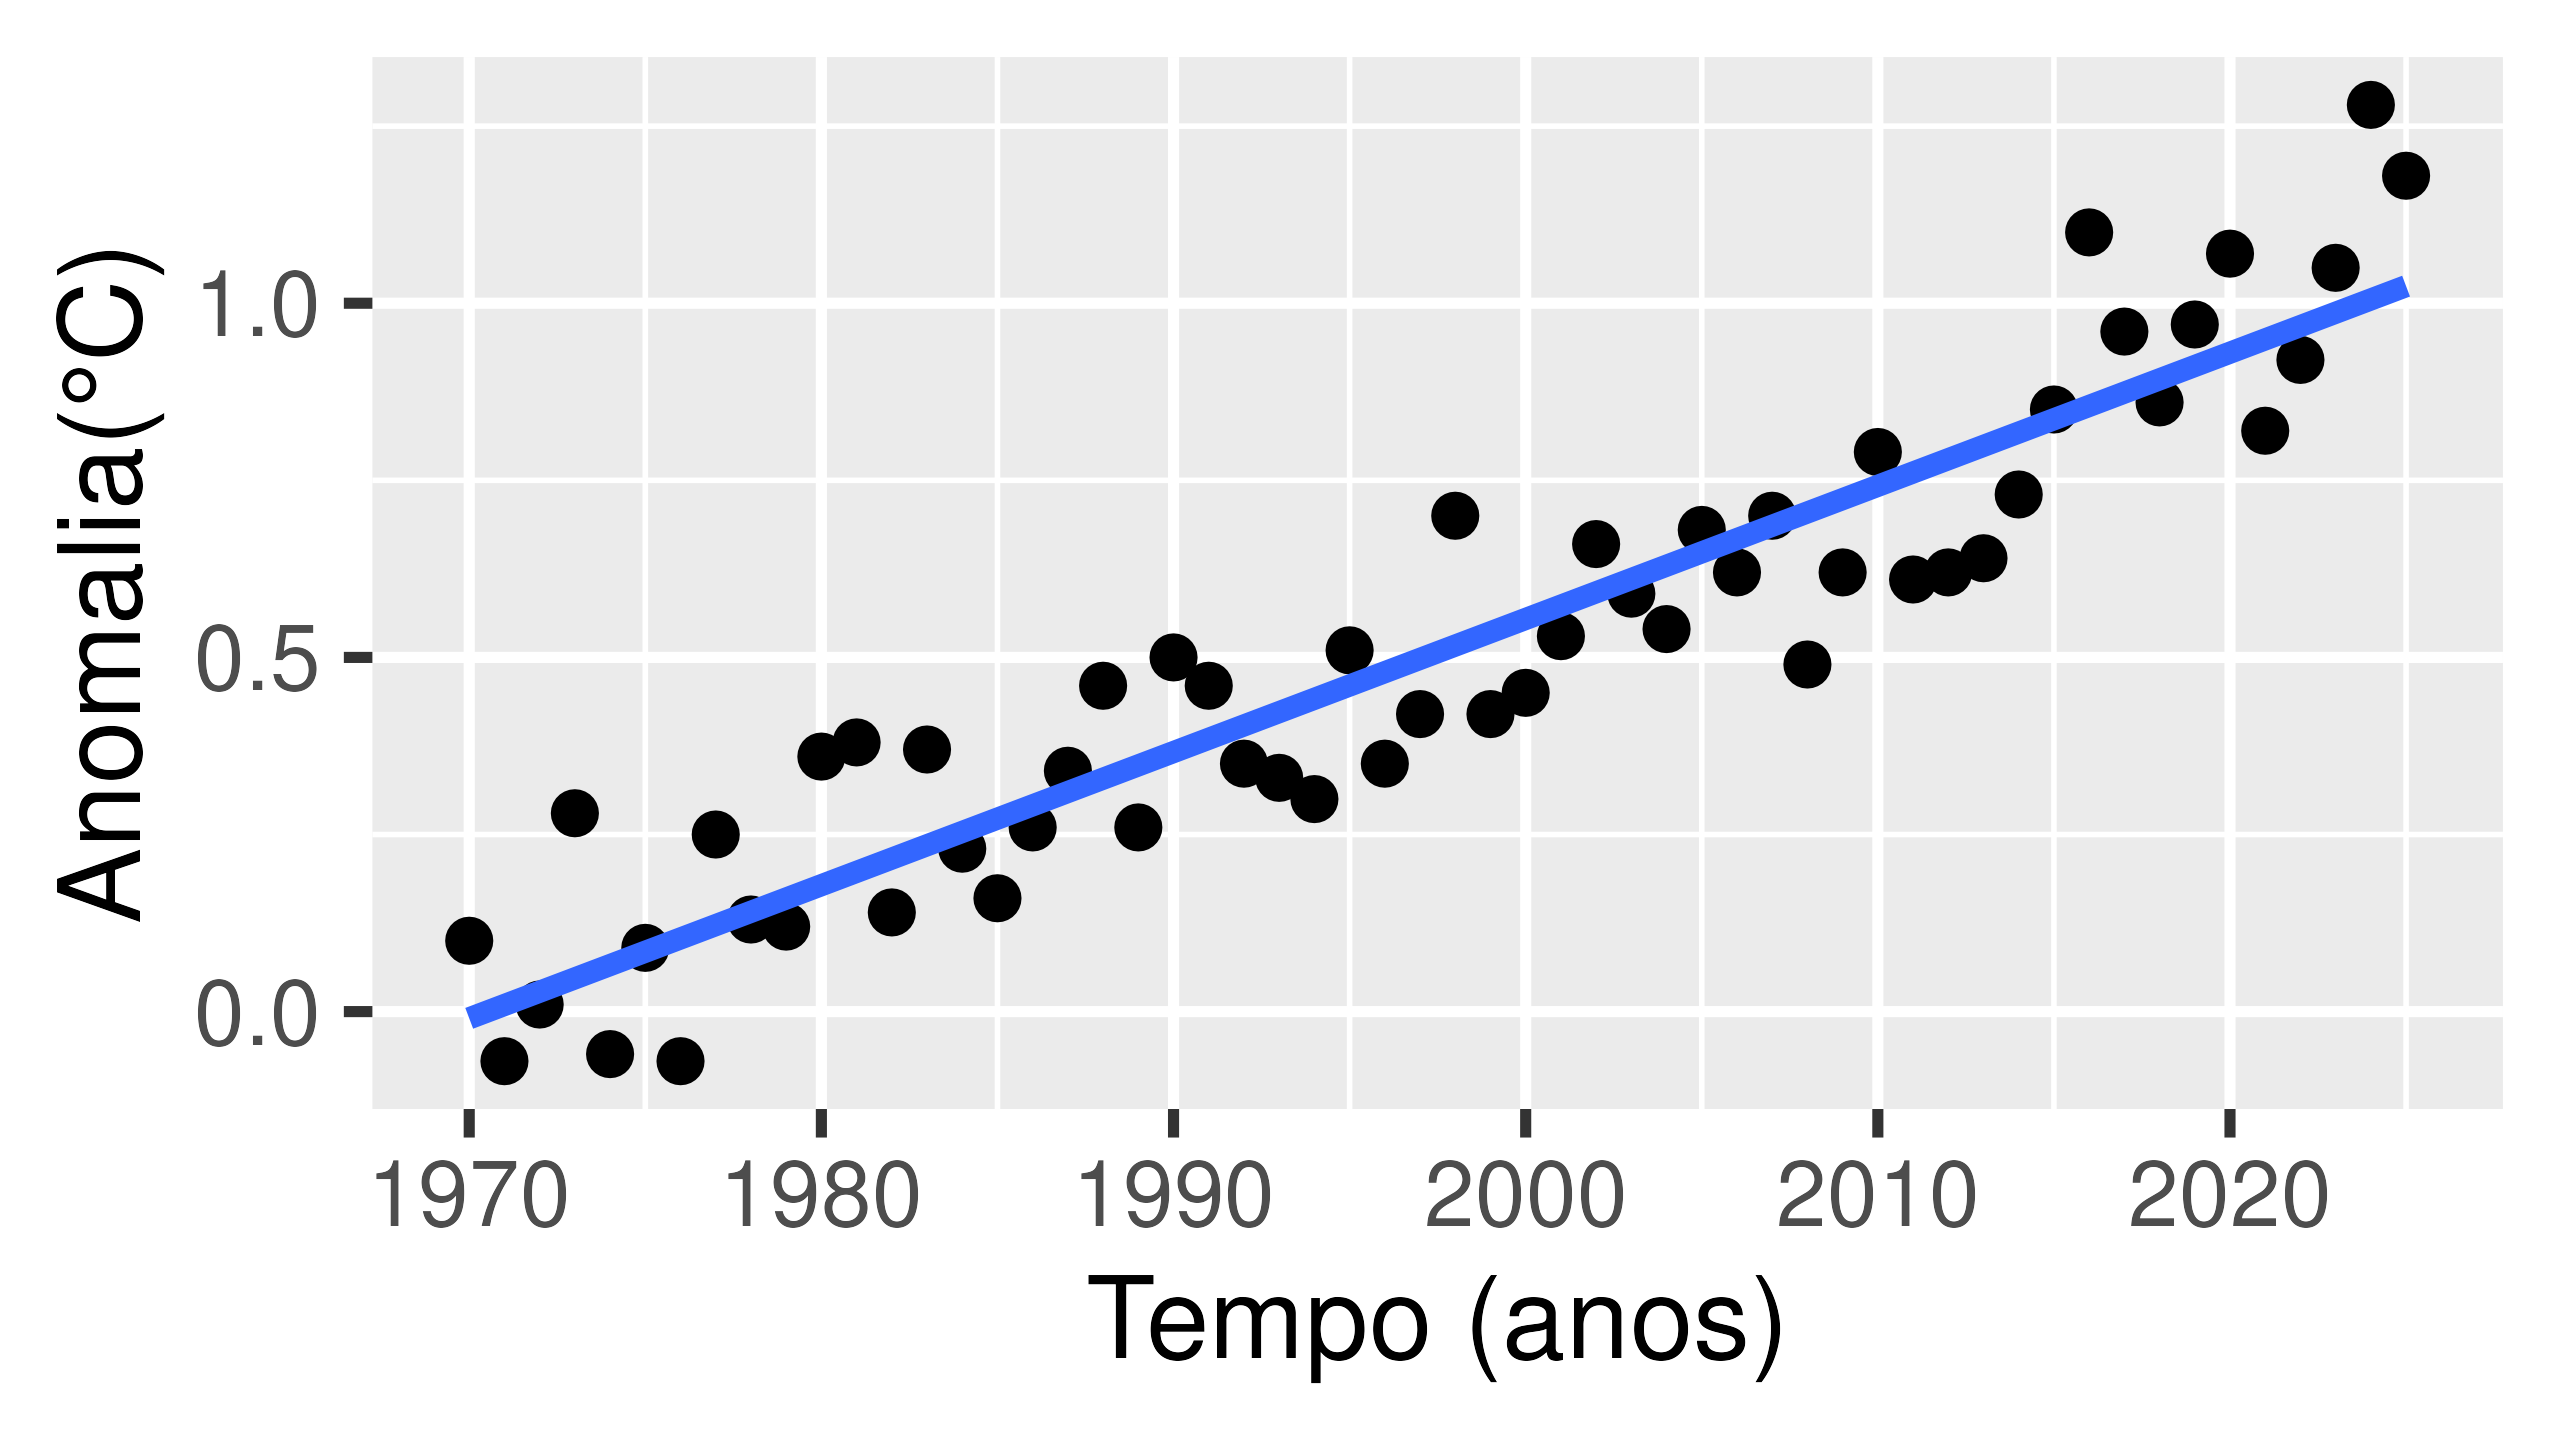
\includegraphics[width=\linewidth]{static/R/plot/anom-3-scatter+reg.png}
    \label{fig:2:anom-3-scatter+reg}
\end{figure}

Antes, foi dito que $\beta_1$ representava a inclinação da reta.
Além disso, ele cumpre uma outra função importante: representar a \textit{taxa de variação} da reta; como a unidade de medida em questão é anos, isso significa quanto a temperatura vai variar por ano.
A regressão realizada nesse conjunto de dados revela que a anomalia de temperatura média global cresce em um ritmo de $0,01879 °C$ ao ano.

Perceptivelmente, essa anomalia vem crescendo mais nos últimos anos do que vinha anteriormente, devido às mudanças climáticas.
O modelo de reta, por ter que simplificar drasticamente, é incapaz de expressar isso, de tal modo que nos últimos três anos sua estimativa está abaixo do valor real.
Geralmente, o que importa não é o quão próximo o modelo está dos dados já existentes, mas sim o quão bem o modelo se dá com extrapolar esses dados e, literalmente, prever o futuro.
Dadas essas tendências recentes, esse modelo pode não ser tão útil, uma vez que não detêm a habilidade de contemplá-las suficientemente.
Um modelo melhor, nesse caso, ao invés de uma reta usaria uma curva.
Um exemplo está na figura \ref{fig:2:anom-3-scatter+reg+poly}.

\begin{figure}
    \centering
    \caption{Gráfico da anomalia (°C) em função do tempo (anos), 1970-2025, com regressão linear e aproximação polinomial}
    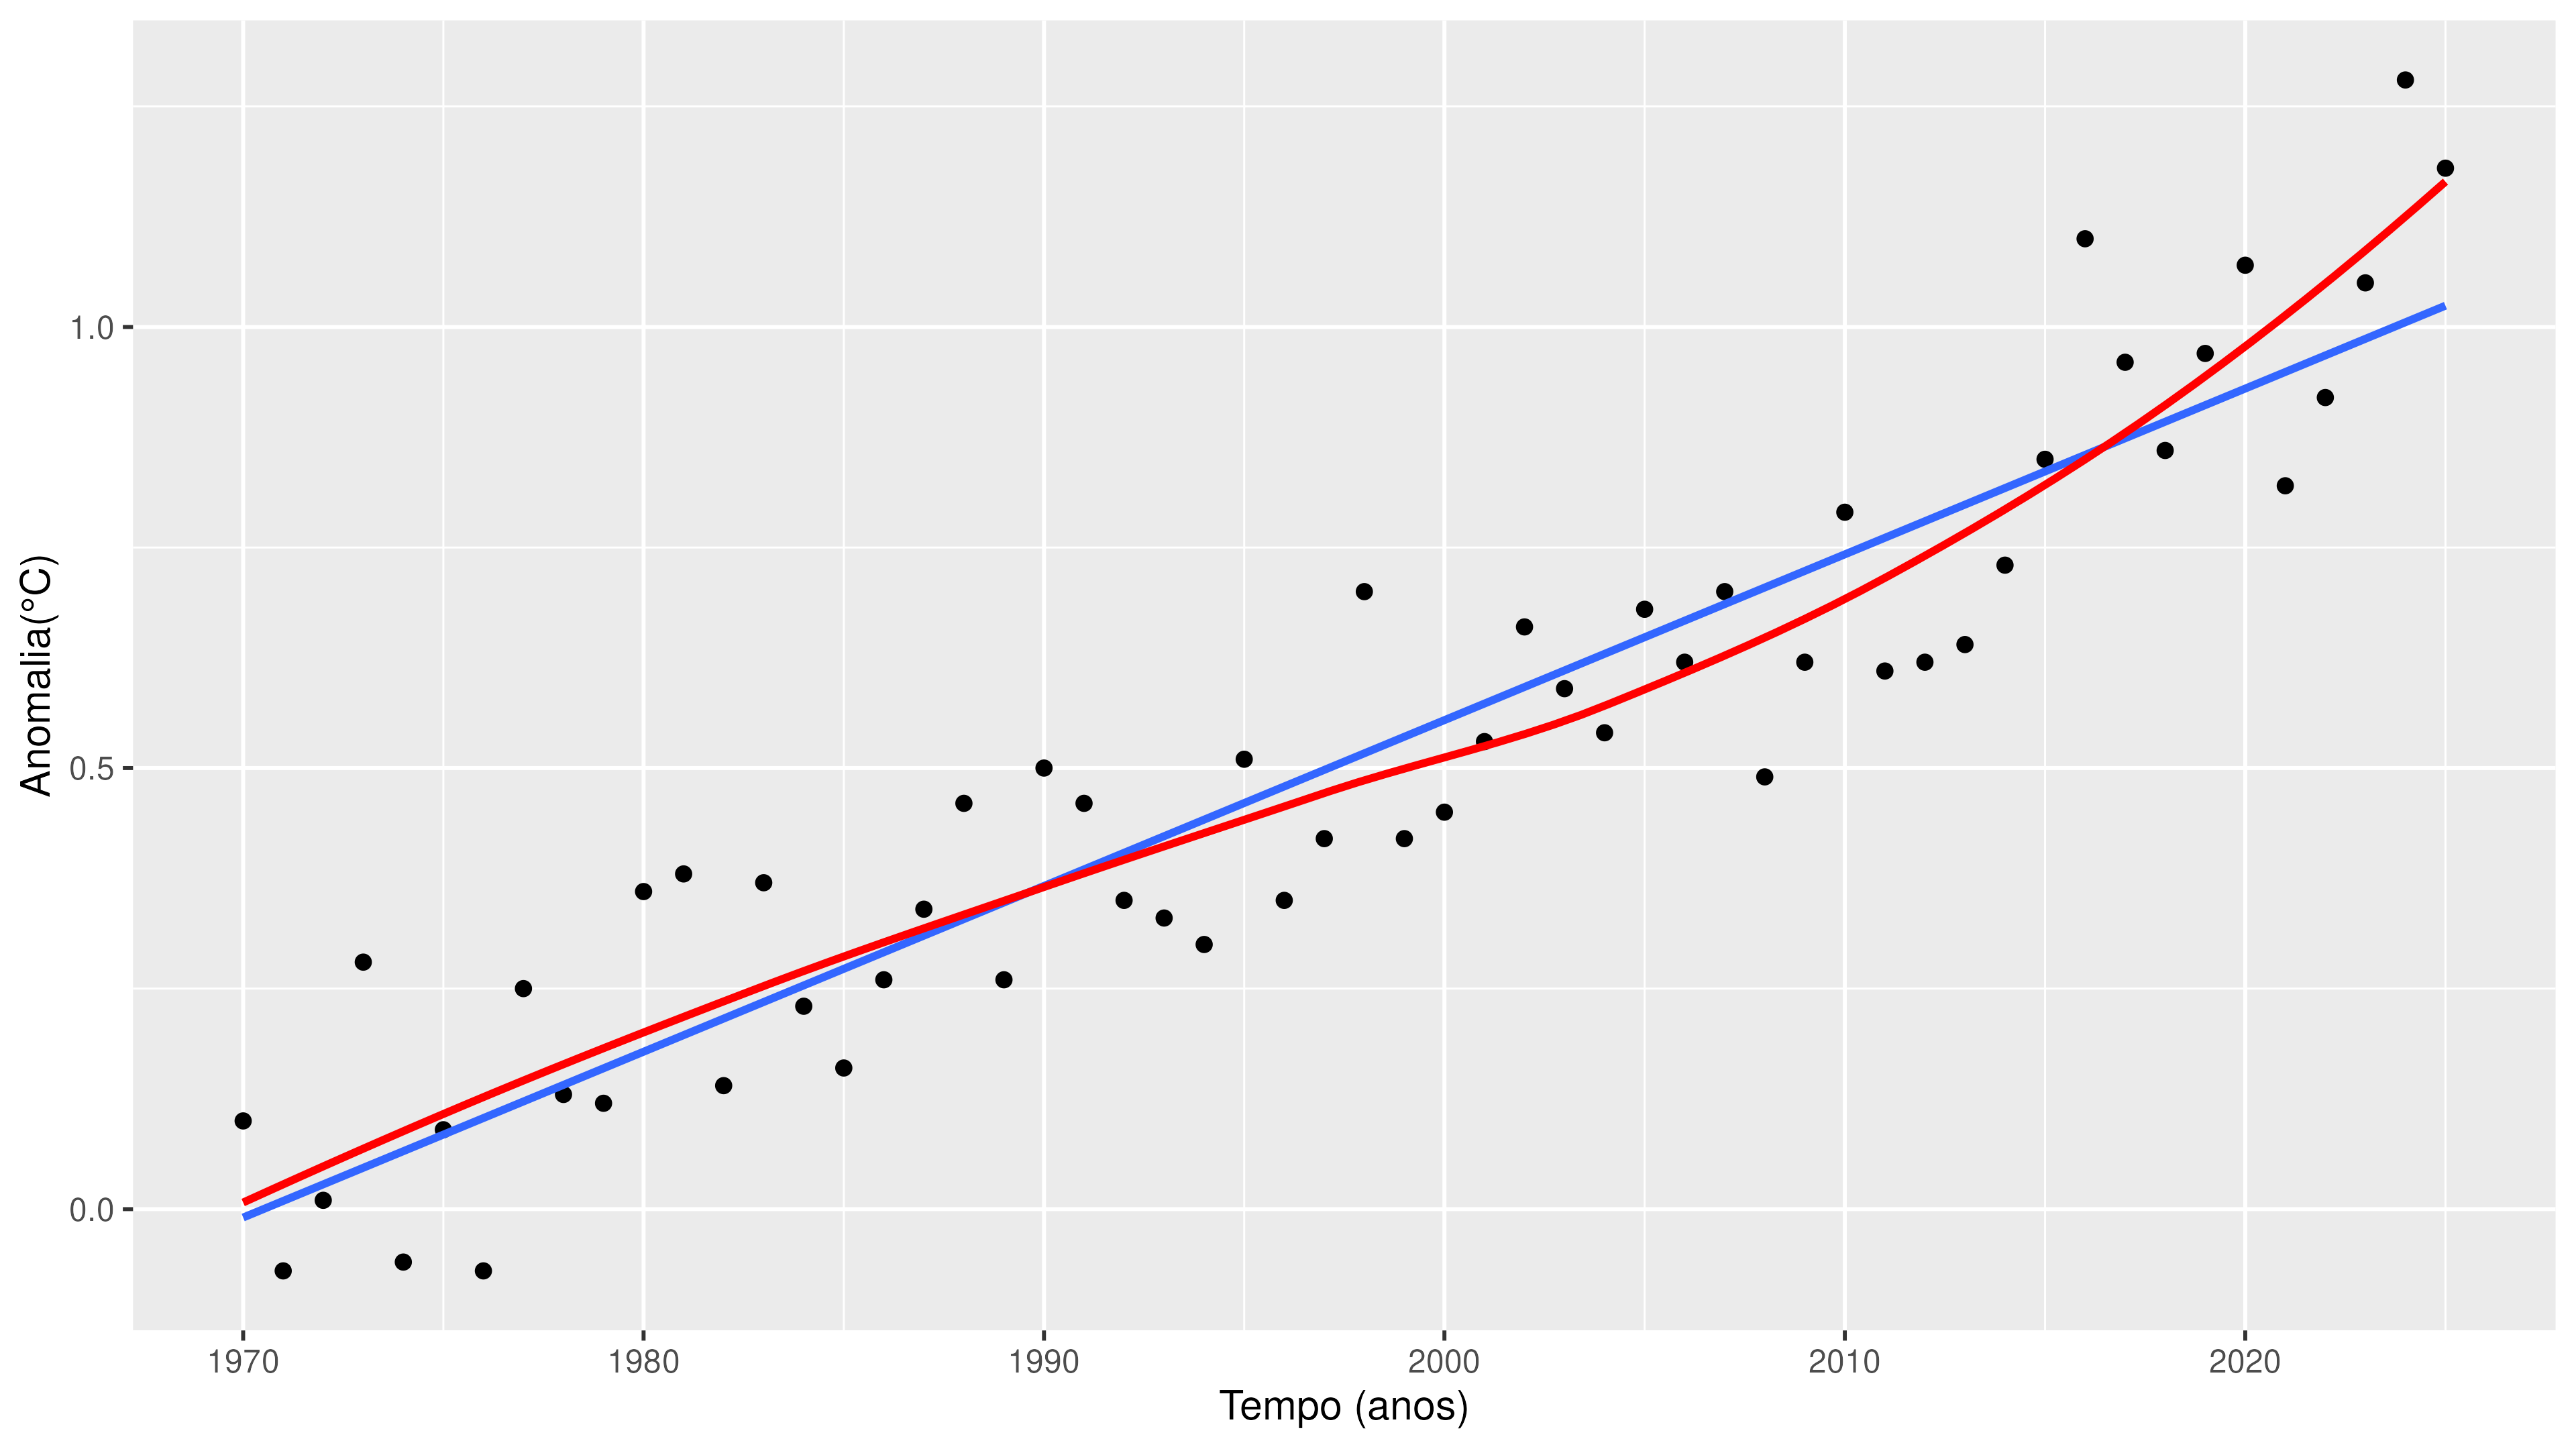
\includegraphics[width=\linewidth]{static/R/plot/anom-5-scatter+reg+poly.png}
    \label{fig:2:anom-3-scatter+reg+poly}
\end{figure}

Esses modelo não é mais linear, evidentemente.
É, pelo contrário, uma curva definida por meio de um polinômio.
Nesse caso, a representação matemática está mais aquém de

\begin{equation}
A(t) = \beta_0 + t \beta_1 + t^2 \beta_2 + t^3 \beta_3 \dots t^n \beta_n 
\end{equation}

Onde $n$ é o grau do polinômio a ser criado.
Aqui, não se trata de uma regressão \textit{linear}, mas sim, \textit{polinomial}.

Está além do escopo deste presente texto debater o funcionamento interno desses modelos (isto é, como efetivamente ocorre a regressão linear), mas é importante perceber que, quando se utiliza uma curva, ao invés de uma reta, o modelo torna-se mais flexível, podendo adaptar-se melhor às condições dos dados.
O erro, que debatemos antes, é menor.
Contudo, ao invés de dois parâmetros simples -- $\beta_0$ e $\beta_1$ -- agora há $n$, que não podem ser interpretados de uma maneira tão direta quanto esses dois.
Isto é, ganha-se flexibilidade, mas há uma perda de interpretabilidade.
Na próxima seção, \ref{sec:2:redes-neurais}, será estudado um modelo ainda mais flexível; e ainda menos interpretável
A seção \ref{sec:2:exemplo-real} debaterá como essa ``interpretabilidade'' é refletida em um caso real: é possível pedir explicações desses modelos?
Isto é, determinar porque algo foi classificado como bom ou ruim, A ou B?

O exemplo aqui apresentado parece simples, mas serve para definir um conceito importante, que será retomado múltiplas vezes: o \textit{aprendizado de máquina}.
Para um computador, aprender é diminuir uma função erro, por meio da alteração de um conjunto de parâmetros.
O aprendizado requer dados; muitos dados; e aí entra o conteúdo do primeiro capítulo.
Terminado o treinamento, o modelo vai poder, a partir dos dados coletados, realizar previsões, inferências, classificações, entre outros, acerca desses dados.

Regressões lineares são um dos algoritmos mais simples que demonstram a dinâmica completa do aprendizado de máquina; tanto é, que foi o primeiro desses algoritmos a ser estudado, com o método de mínimos quadrados tendo sido empregado por Isaac Newton para determinar a duração exata do ano \cite{belenkiy_groping_2016}.
Há diversas maneiras de melhorá-lo.
Uma das mais simples é realizar a regressão em mais de uma variável; por exemplo, podemos estimar o preço de uma casa baseado no tamanho (em $\text{m}^2$), o número de quartos, a distância do centro, o andar, e a idade da casa.
O modelo se assemelharia à equação \ref{eq:2:lm-mult}.

\begin{equation}
\label{eq:2:lm-mult}
\text{Preço} = \beta_0 + \beta_1 \cdot (\text{Tamanho}) + \beta_2 \cdot (\text{Quartos}) + \beta_3\cdot (\text{Distância}) + \beta_5 \cdot (\text{Andar}) + \beta_6 \cdot (\text{Idade})
\end{equation}

Onde $\beta_1$, $\beta_2$, $\beta_3$, $\beta_4$, $\beta_5$ e $\beta_6$ representam o quão significativos seus respectivos parâmetros são para o preço total do apartamento.

\section{Redes Neurais}\label{sec:2:redes-neurais}
Por mais úteis que as regressões lineares possam ser, ainda são um modelo rudimentar, que trabalha com alguns pressupostos bastante restritivos.
Um deles é o da linearidade da relação entre uma variável -- como o ano, no caso da anomalia de temperatura, ou o andar, no caso do preço de apartamentos -- e o resultado desejado.
Assim, pressupõe-se que essa relação se dá por uma reta, e não, por exemplo, um curva exponencial, logarítmica, ou qualquer outra coisa que fuja da linearidade.
Viu-se que isso pode ser consertado por meio de uma regressão polinomial\footnote{A regressão polinomial está associada à muitos outros métodos que a acompanham. Para estendê-la para uma predição com base em multiplas variáveis, como na equação \ref{eq:2:lm-mult}, por exemplo, é possível usar um Método Aditivo Generalizado (GAM). Os GAMs estabelescem uma função polinomial de grau $n$ \textit{para cada variável}, ou seja, uma função para o tamanho, uma para o número de quartos, uma para a distância do centro, e por aí vai. Assim, o modelo toma a cara de $\text{Preço} = \beta_0 + f_1(X_1) + f_2(X_2) + f_3(X_3) + \dots + f_i(X_i)$, onde $X_1\dots X_i$ são as variáveis (como o andar e o número de quartos) e $f_1\dots f_i$ são as funções de grau $n$ que dependem de cada variável \cite{james_introduction_2021a}}.
Contudo, há ainda um problema maior que impede-a de ser utilizada em mais contextos: a possiblidade de relações entre variáveis.
Para entender o que isso significa, considere um outro exemplo: o banco de dados MNIST \cite{lecun_mnist_}.

Ele é composto por milhares de imagens de dígitos de 0-9 desenhados à mão, assim como na figura \ref{fig:2:mnist}.
O objetivo que ele apresenta é fazer um modelo computacional capaz de identificar os dígitos baseando-se nas imagens apresentadas, semelhante ao que um ser humano faria ao ler esses números.
Por mais que isso pareça simples, esse problema não o é -- as imagens variam muito em sua forma, e a computação demorou para desenvolver métodos flexíveis o suficiente para essa tarefa.

\begin{figure}[H]
\caption{Algumas imagens do banco de dados MNIST}
\centering
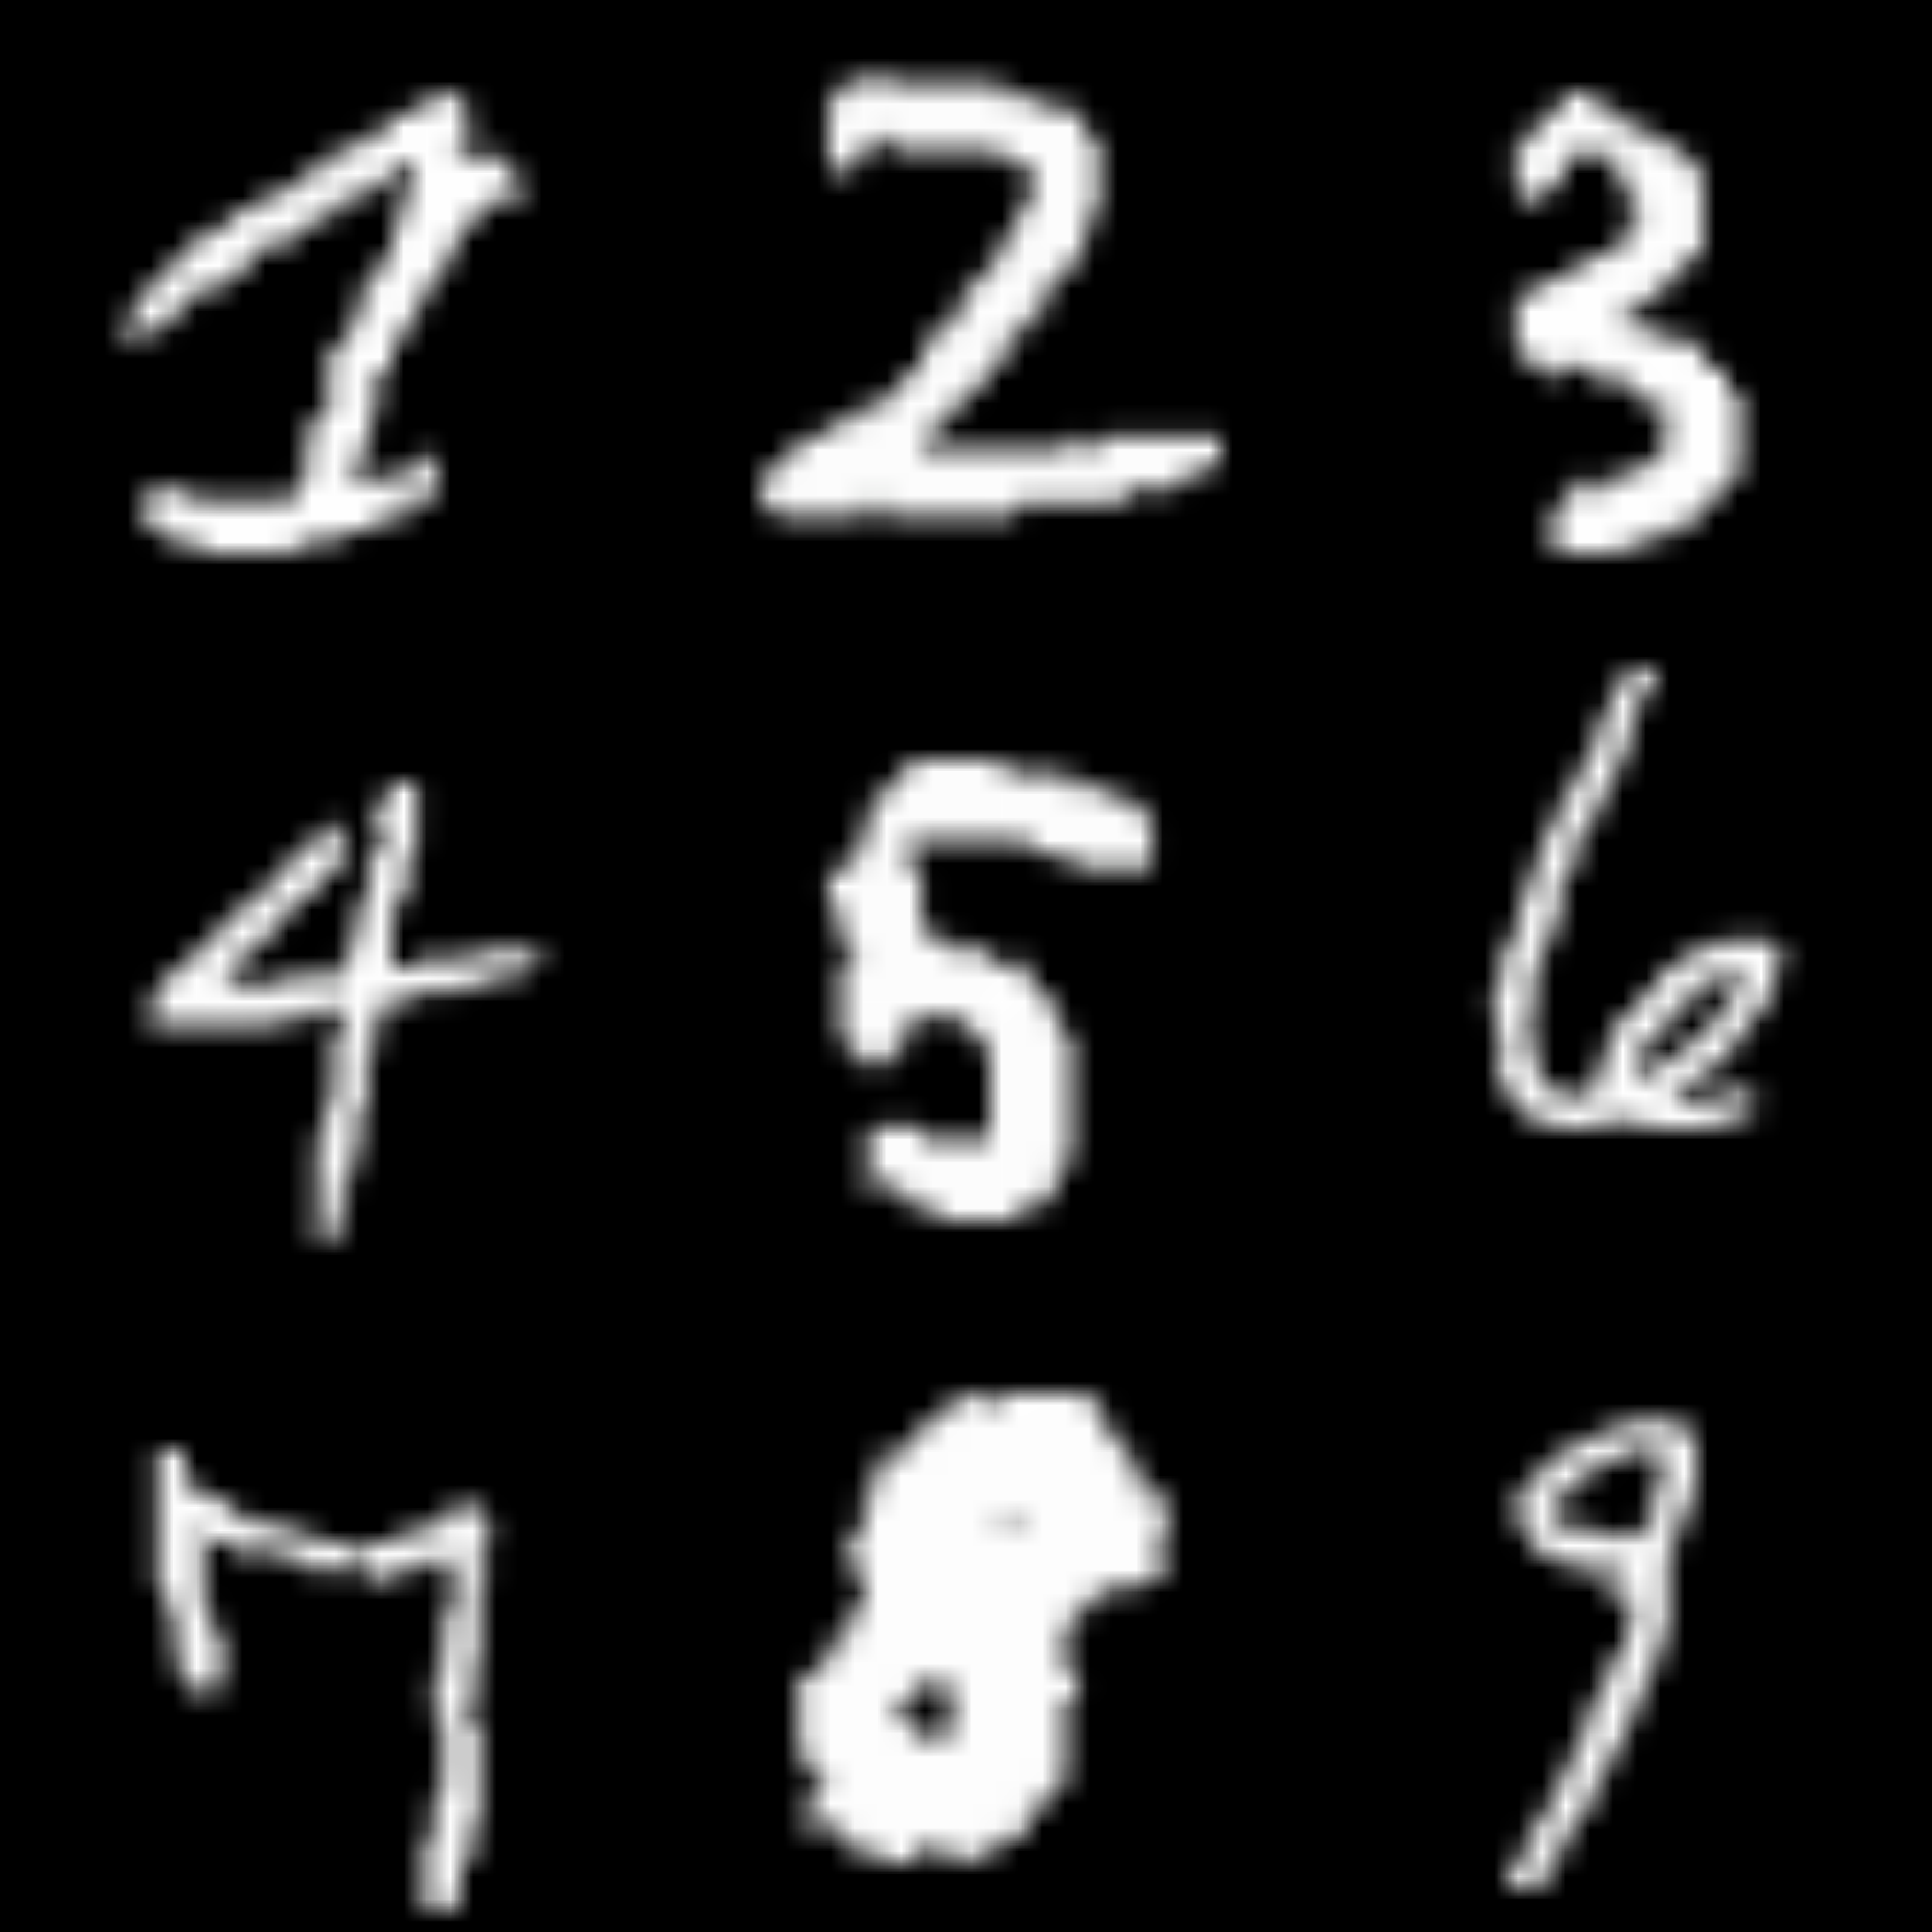
\includegraphics[width=0.5\linewidth]{static/MNIST.png}
\label{fig:2:mnist}
\end{figure}

O banco de dados MNIST foi publicado em 1998, e, segundo o próprio autor, o recorde é de $0,23\%$ de erro, atingido em 2012, dentre os resultados publicados na literatura \cite{cireşan_multicolumn_2012}.
As primeiras tentativas resultaram em taxas por volta dos $12\%$ \cite{lecun_mnist_1998}.
\section{O Mundo Real}\label{sec:2:exemplo-real}
\section{Natureza}


\addcontentsline{toc}{chapter}{Referências}
\printbibliography
\end{document}
